\documentclass[authoryear, 12pt,5p, times]{elsarticle}
%\usepackage[hypcap]{caption}
%\geometry{margin=0.95in,top=1.4in,bottom=1.4in}
\geometry{margin=1.1in,top=1.5in,bottom=1.5in}
\usepackage{float}
\usepackage{amsmath}
\usepackage[hidelinks]{hyperref} 
 \usepackage{gensymb}
\usepackage{subcaption}
\usepackage{url}
%\renewcommand\thefootnote{\fnsymbol{\dagger}}
\usepackage[symbol*]{footmisc}
\makeatletter
\newcommand{\rpm}{\raisebox{.3ex}{$\scriptstyle\pm$}}
\begin{document}
%\footnote{This is a footnote}
\begin{frontmatter}
\title{Introductory Experiments and Linear Circuits I}
\author{\today \quad \\Jung Lin (Doris) Lee [Lab Partner: Leah Tom]\\Prof. William Holzapfel, GSI Thomas Darlington, Thomas Mittiga, John Groh,  \\Victoria Xu, Jonathan Ma, Francisco Monsalve, Xiaofei Zhou}
	\begin{abstract}
 ----------
	\end{abstract}
\end{frontmatter}
\section{Introduction} 
 \section{Keithley 2110 Digital Multimeter3 (DMM)}
%- uncertainty
%The range should be adjusted  suitable range within --- for each measurement , within order of magnitude. \footnote{Too large a range will result in the error ``OVLRD" (overload) and too low will cause ---}
\section{BSC Laboratory Breadboard Box}
\begin{figure}[h!]
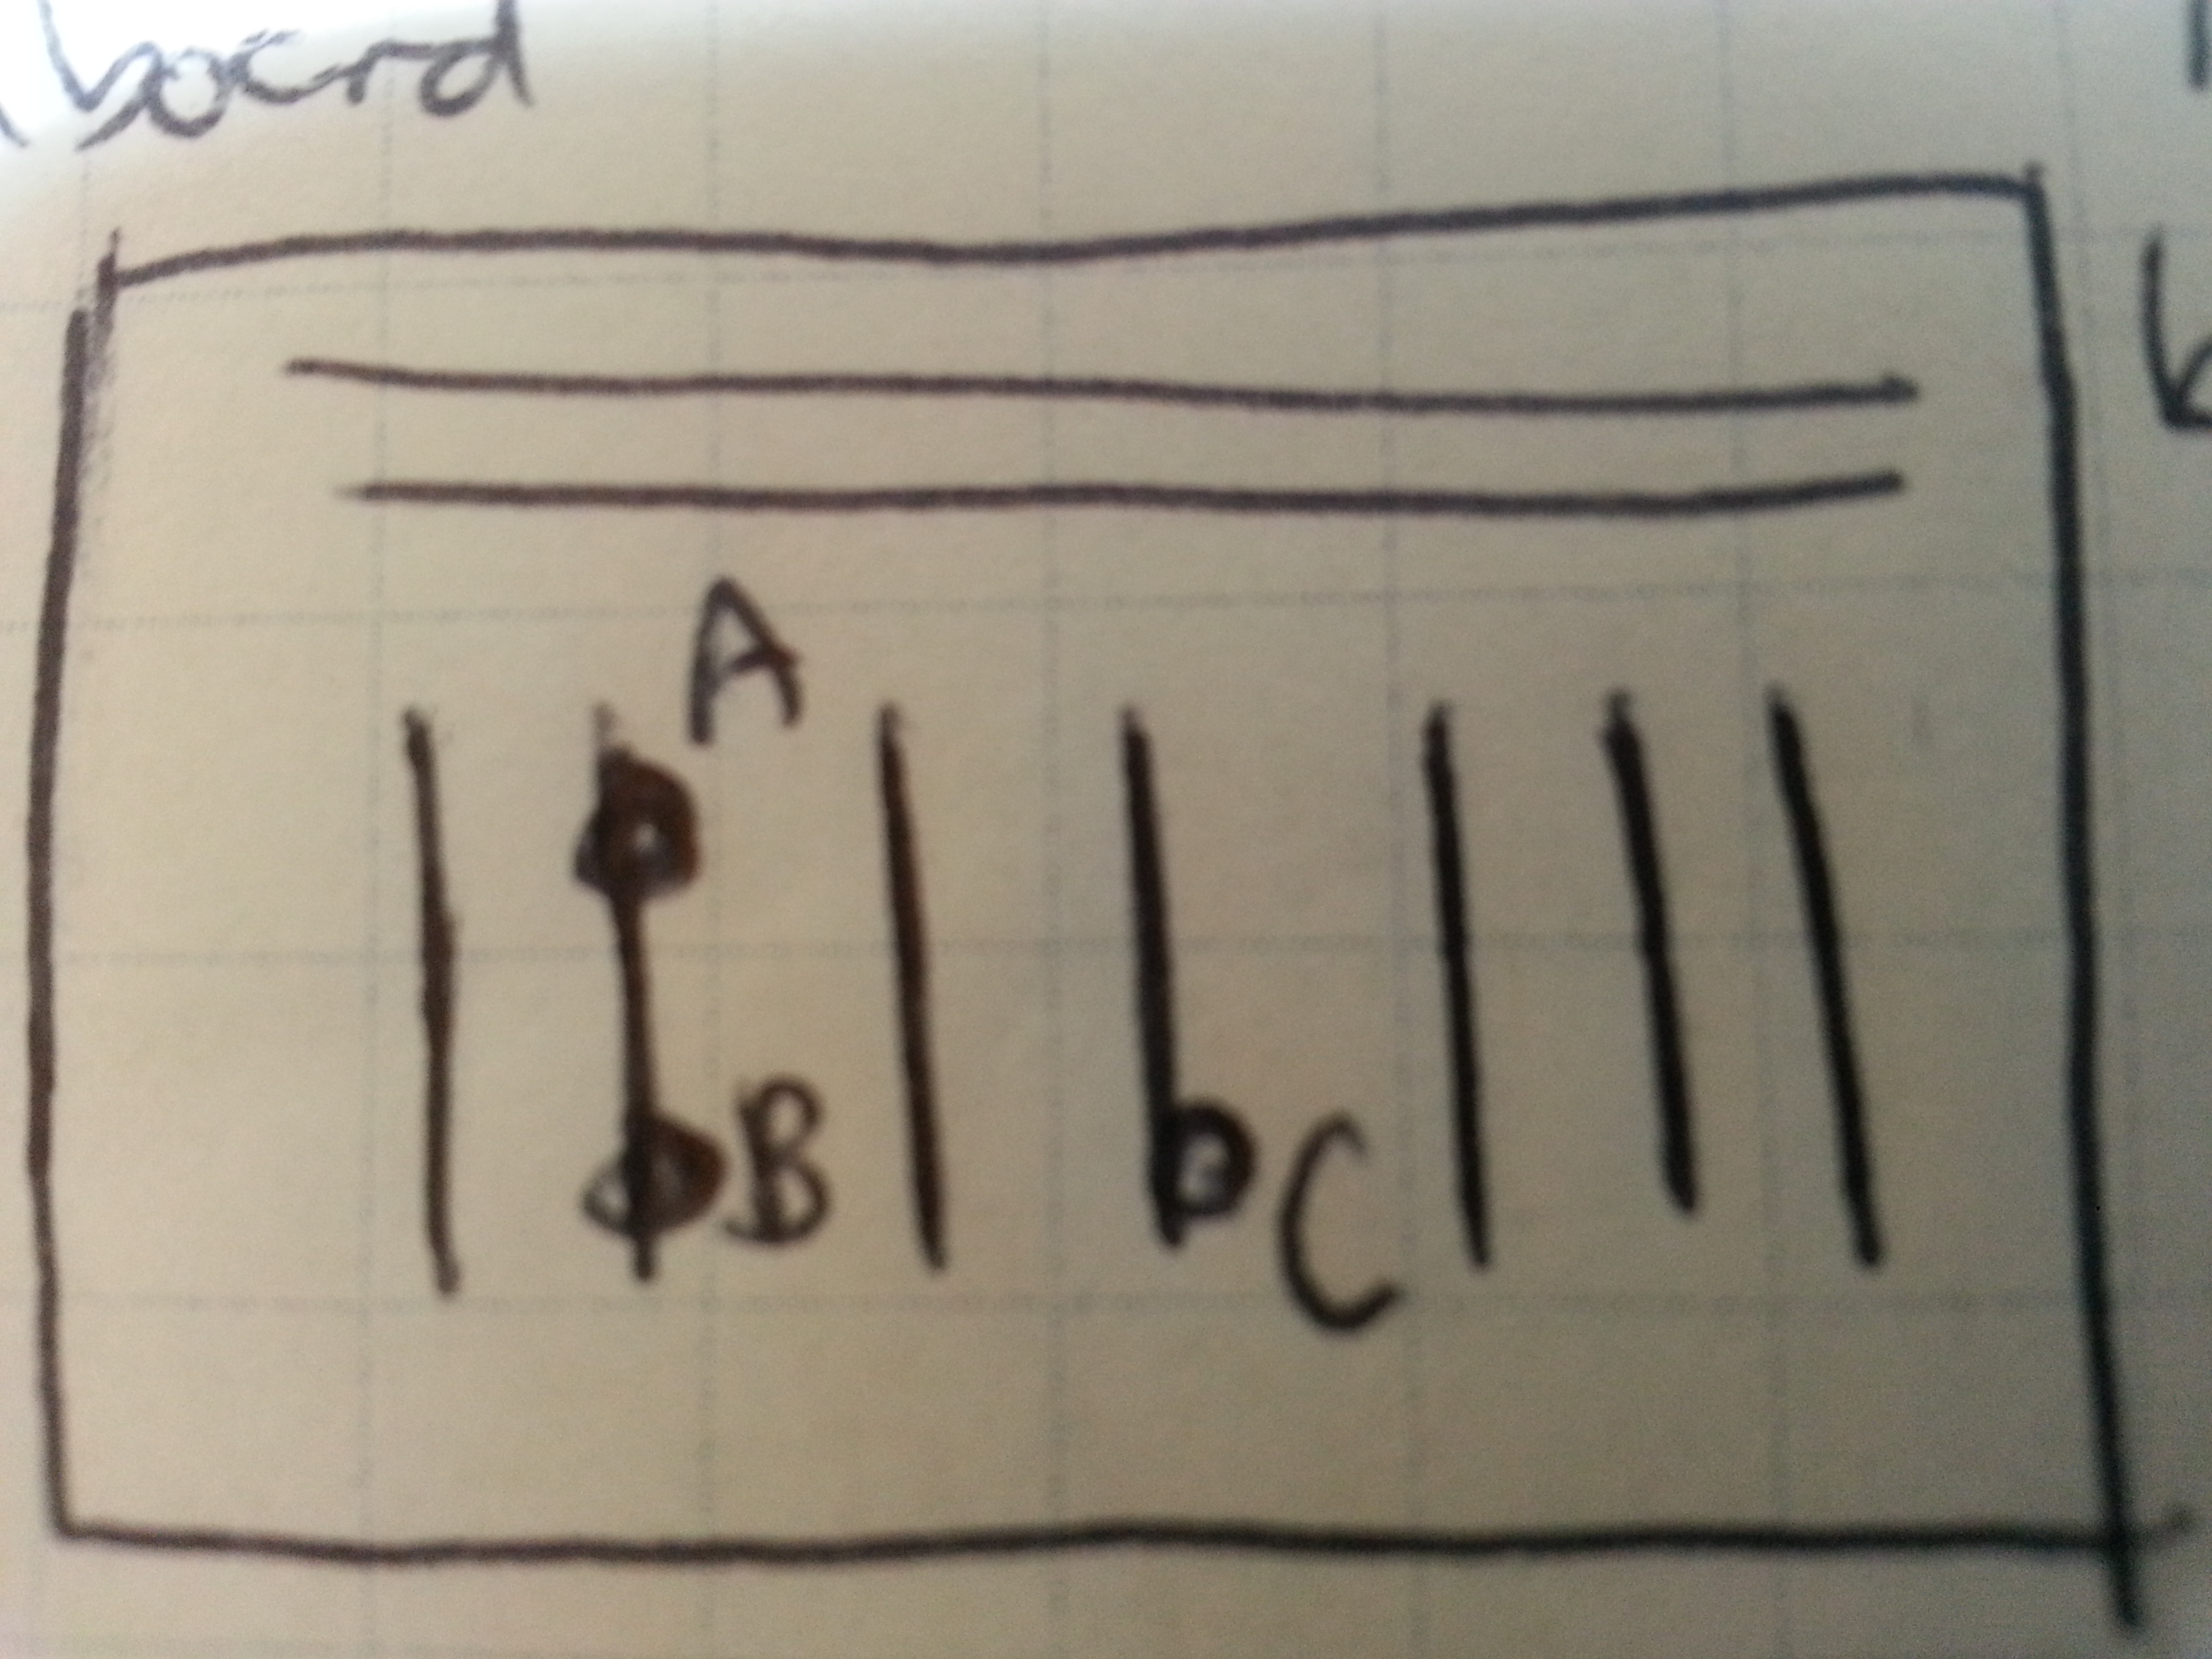
\includegraphics[width=0.5\textwidth]{figure/d_breadboard}
\caption{We put jumper wires connecting the A and B, B and C separately and measure the resistance across them.}
\label{breadboard}
\end{figure}
\paragraph{\textbf{1.1}}
The breadboard is a device suitable for rapid-protoyping circuits, without long chemical etching process of the PCB.  As shown in Fig.\ref{breadboard} , it is horizontally connected along the longer edge for the two top and bottom buses, which often serves as to input voltage and grounding --. We measured the resistance across A and B as 0.16 $\Omega$ and across B and C as ``overload".  These result make sense because since B and C is not connected, the resistance is almost infinite, and is therefore not registered on the DMM. Likewise, since A and B are connected, there is minimal resistance between them.
\paragraph{\textbf{1.3}} 
The reading between the 12 output and the 5V supply ground fluctuates around 0V. The reasoning behind this result is that the 12V terminal and 0V pair only supply a 12V potential difference with respect to ground. However, the common and the ground is not necessarily at the same potential.  If the common and ground is not connected, we must consider the left and right voltage terminals in Fig. \ref{ground_common} as distinct. Therefore, connecting the 12V and 5V terminal essentially brings them both to equipotential, resulting in a potential difference of $\approx$  0V.
\begin{figure}[h!]
\center
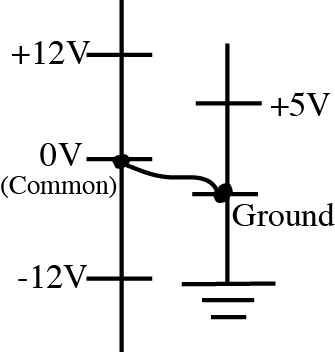
\includegraphics[width=0.25\textwidth]{figure/ground_common}
\caption{By connecting the ground to the common, we can set both the 12V and the 5V with respect to ground, thereby creating the 17V output voltage.}
\label{ground_common}
\end{figure}

%%%%%%%%%%%%%%%%%%%%%%%%%%%%%%%%%%%%%%%
\paragraph{\textbf{1.5}} \label{1_5}
Since the resistors are arranged in series as shown in Fig.\ref{voltage_divider}, the current through each resistor should be the same.  
\begin{equation}
I=\frac{V}{R_{eq}}=\frac{V}{R_1+R_2}=\frac{24V}{480k\Omega
}= 5.0\times10^{-5}A 
\end{equation}

%%%%%%%%%%%%%%%%%%%%%%%%%%%%%%%%%%%%%%%%
\paragraph{\textbf{1.7}} 
\begin{figure}[h!]
\center
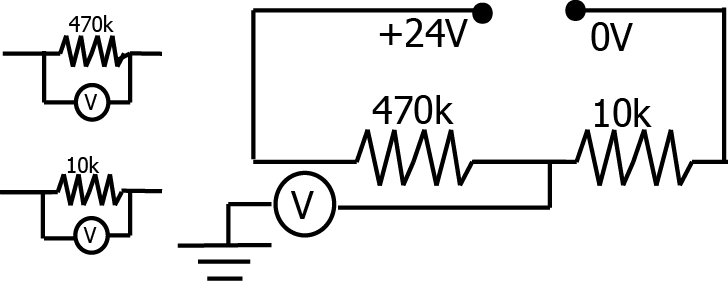
\includegraphics[width=0.5\textwidth]{figure/1_7_setup}
%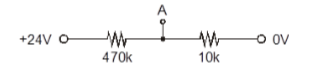
\includegraphics[width=0.25\textwidth]{figure/d_voltage_divider}
\caption{The voltage divider setup for this experiment.}
\label{voltage_divider}
\end{figure}
a) Depending on the DMM setup, it can act as a voltmeter or ammeter. To meaaure the current through a 10k$\Omega$ resistor, we need to connect the DMM in parlalle with the 10k$\Omega$ resistor as shown in Fig. ---- 
Then, using Ohm's law we can compute the current flowing through the 10k$\Omega$ resistor: 
\begin{equation}
I = \frac{V}{R}=\frac{0.510V}{10k\Omega}=5.1\times 10^-5 A
\label{current}
\end{equation}
which is approximately the same as predicted in \ref{1_5}. Alternatively, we can also connect the DMM in series with the resistor as shown in the top right figure of Fig. \ref{voltage_divider}  to measure the current directly, and this yields the same current value as computed in Eq.\ref{current}.\footnote{Note that the ground and sensing probes need to be plugged into a different set of holes instead of the two terminals plugged in for the voltage measurement. Both the upper pairs will work but the upper left pairs  gives a more precise reading.} 
\\
b)  We connected the DMM across the  470k$\Omega$ resistor as show in the lower left figure in Fig. \ref{voltage_divider} and obtained a reading of 24.079V, with the range set as 10V. Using Eq. \ref{accuracy1_7}, we compute the actual reading range as 24.079V $\pm $3.29mV:
\begin{equation}
0.012\% \times 24.079V+0.004\%\times 10V=3.28948mV
\label{accuracy1_7}
\end{equation}

%%%%%%%%%%%%%%%%%%%%%%%%%%%%%%%%%%%%%%%%
\paragraph{\textbf{1.9}} 
The current through each resistor is: 
\begin{equation}
I = \frac{24.589V}{(465.6+9.89)k\Omega} = 0.0517mA
\end{equation}
There is a 0.17\% deviation from the nominal values computed in \ref{1_5}.
Using Eq. (----REF Eq. in \#1.4--!!!), the voltage at point A is computed as: 
\begin{equation}
V_A= \frac{24.589V \times 9.89k\Omega}{(465.6+989)k\Omega} = 0.5114V
\end{equation}
Comparing this result with values from (REF 1.6!!), there is a 1.14\% error.

%%%%%%%%%%%%%%%%%%%%%%%%%%%%%%%%%%%%%%%%
\paragraph{\textbf{1.11}}
\begin{equation}
I_{\text{through }R_1} = 24.072V 
5.1217\times10^-5A
\end{equation}

The current measured directly by the DMM is 0.0030 mA. 
\section{Digital Oscilloscope}
%voltage on the vertical axes and time on the horizontal axes
%\subsection{Tune-able Parameters and useful functions}
%\begin{itemize}
%\item AC/DC Setting : (See Sec.\ref{sec:acdc})
%\item Scale: Vertical and horizontal zoom in ; adjust accordingly to --- window that best captures
%\item Measurement: useful quantities 
%\end{itemize}
\section{Frequency and time measurements}
%%%%%%%%%%%%%%%%%%%%%%%%%%%%%%%%%%%%%%%%
\paragraph{\textbf{1.17}}
a) We measured the voltage measurement as 5.0488V and the error on the measurement is computed by: 
\begin{equation*}
0.012\%(5.0488V)+0.004\%(10V) = 1.0059V
\end{equation*}
\par b) We adjusted the settings of the oscilloscope to add the  measurement of the mean and amplitude and obtained a reading of 4.984V and 240.0 mV respectively. Since our signal is a flat line on a V-t graph, the fluctuation on the y axes informs us about how the voltage changes in time. The amplitude is the variance on the averaged voltage value that we obtained, and therefore serves as an estimate for the error our voltage measurement. 
\par
c) We find that as we decrease the voltage per division, our amplitude (estimated error) also decreases. The more refined division of the voltage values scale results in greater precision of the measurement, analogous to how the range of our DMM must be adjusted to minimize the uncertainty of the  measurement.
\par
d) The best scope setting is the 1V/div since yields the smallest variance. \footnote{Any settings for 1V/div  or below is not accurate enough  for the oscilloscope to conduct a measurement since the time averaging window does not contain all  of the signal . For example, the 500mV/div setting yields a variance of $>$2.56V, which is over 50\% error relative to the actual value.}


%%%%%%%%%%%%%%%%%%%%%%%%%%%%%%%%%%%%%%%%
\paragraph{\textbf{1.19}} 
The root mean square voltage ($V_{rms}$)is often given as a useful quantity for finding the power. The $V_{rms}$ is defined by the root of the time-averaged,squared voltage as:
\begin{equation}
V_{rms} = \sqrt{\frac{1}{T}\int_0^{t_0} V_s(t) ^2 dt} 
\end{equation}
$\text{Let us define} V_0 = \text{Amplitude}$,\footnote{The ``amplitude" measurement option of the oscilloscope defines its readings as 2$V_0$, a value close to the $V_{pp}$ reading.}$V_{pp} =  $Peak-to-peak voltage= 2$V_0$ , $V_s$= signal's voltage. 
\par  a) For a sine wave signal, the $V_{rms}$ is computed by: 
\begin{align}
V_{rms} = V_0\sqrt{ \frac{1}{2\pi}\int_0^{2\pi}sin^2 x}= \frac{V_0}{\sqrt{2}}
\end{align}
\par b) For a triangular wave signal, we can simply compute over 1/4 of its period, since the area under the signal in that interval is the same (i.e. power and $V_{rms}$): 
\begin{align}
V_{rms} = \sqrt{ \frac{4}{T}\int_0^{\frac{\pi}{2\omega}}\Bigg(\frac{V}{\pi/2\omega}\Bigg)^2 xdx}=\frac{V_0}{\sqrt{3}}
\end{align}
\par c) Geometrically, we can see that the $V_{rms}$ of a square wave signal is equal to its $V_0$.
We measure the V$_0 $, V$_{pp}$, V$_{rms}$ of a input signal on the oscilloscope, as shown in Table \ref{Vrms_table}. 
%\footnote{Uncertainty computed by Eq.\ref{accuracy1_7}}.
\begin{table}
    \begin{tabular}{l|l|l|l}
    Type       & V$_0 $(mV) & V$_{pp} (V)$ & V$_{rms}(mV)$ \\ \hline
    sine       & 496   & 1.02      & 351        \\
    square     & 490   & 1.68      & 490        \\
    triangular & 510    & 1.04      & 283        \\
    \end{tabular}
\caption{Experimental values for oscilloscope measurements. The $V_{rms}$ computed in parts a, b, and c is 361, 485, 255 mV, respectively, which is within 10\% of experimentally obtained values.}
    \label{Vrms_table}
\end{table} 

%%%%%%%%%%%%%%%%%%%%%%%%%%%%%%%%%%%%%%%%
\paragraph{\textbf{1.21}} 
\begin{figure*}[t]
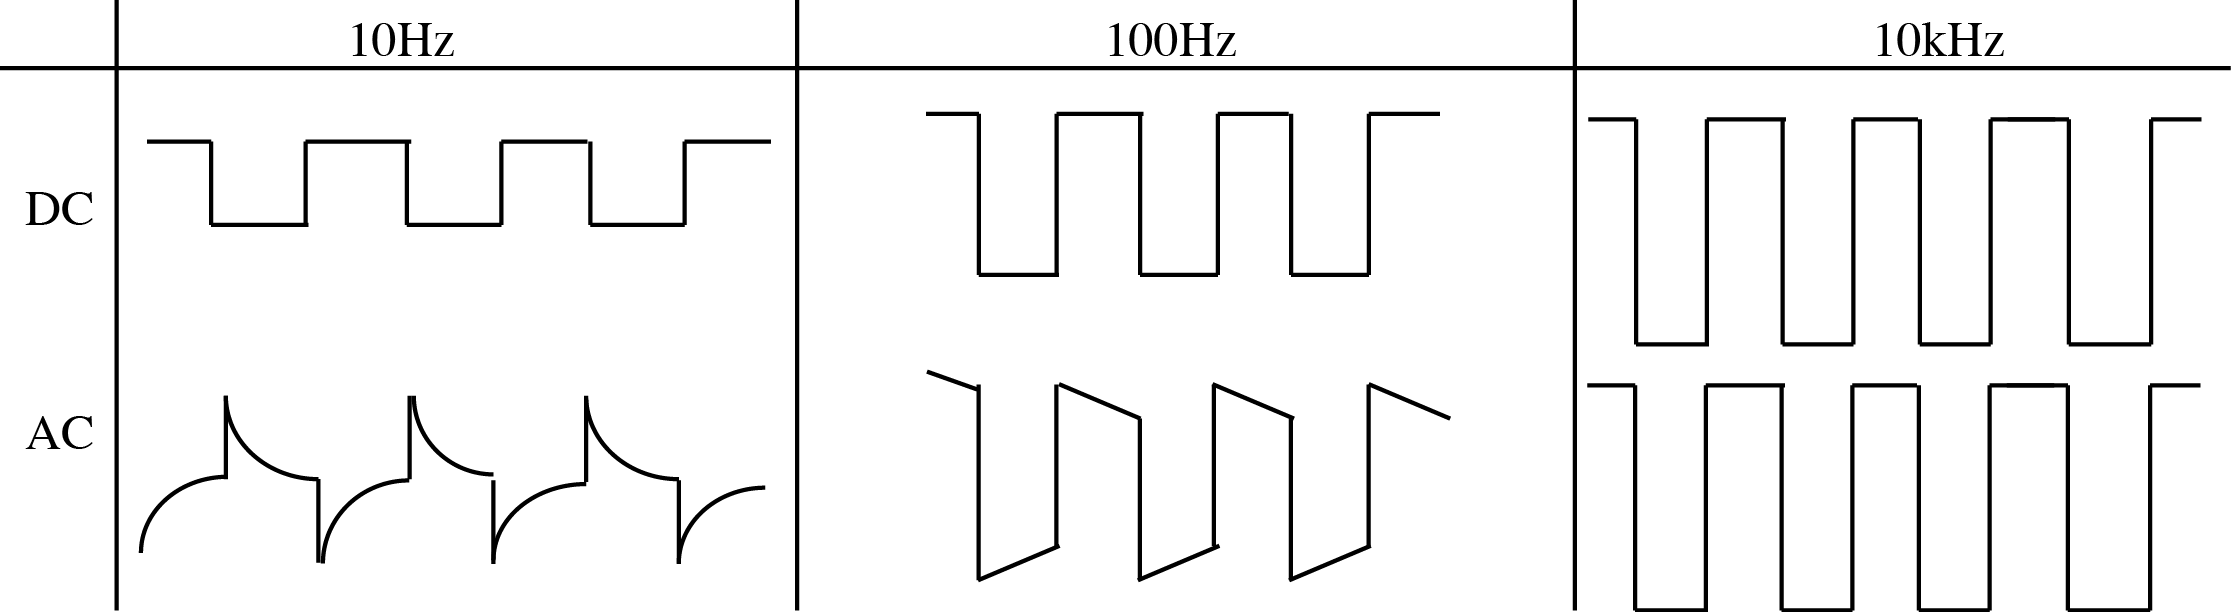
\includegraphics[width=\textwidth]{figure/ACweird}
\caption{At low frequencies, the AC scope traces on the oscilloscope experience distortion.}
\label{AC_weird}
\end{figure*}
The AC setting on the oscilloscope subtracts off the average value from the DC signal. This average is taken over some fixed time interval. So by decreasing the frequency, there will be fewer cycles in the same amount of sampling time, therefore the computed average will be less accurate. Subtracting off such a value yields the sloped wedges seen in 10 and 100 Hz  AC scope traces, as shown in Fig. \ref{AC_weird}.\footnote{Note that the 50$\Omega$ terminator introduces noise to to the scope reading. Therefore, we replaced the terminator component with the ``High Z" setting load on the signal generator.}

\section{Thévenin Analysis}
%%%%%%%%%%%%%%%%%%%%%%%%%%%%%%%%%%%%%%%%%%
\paragraph{\textbf{2.1}}
\begin{figure}[h!]
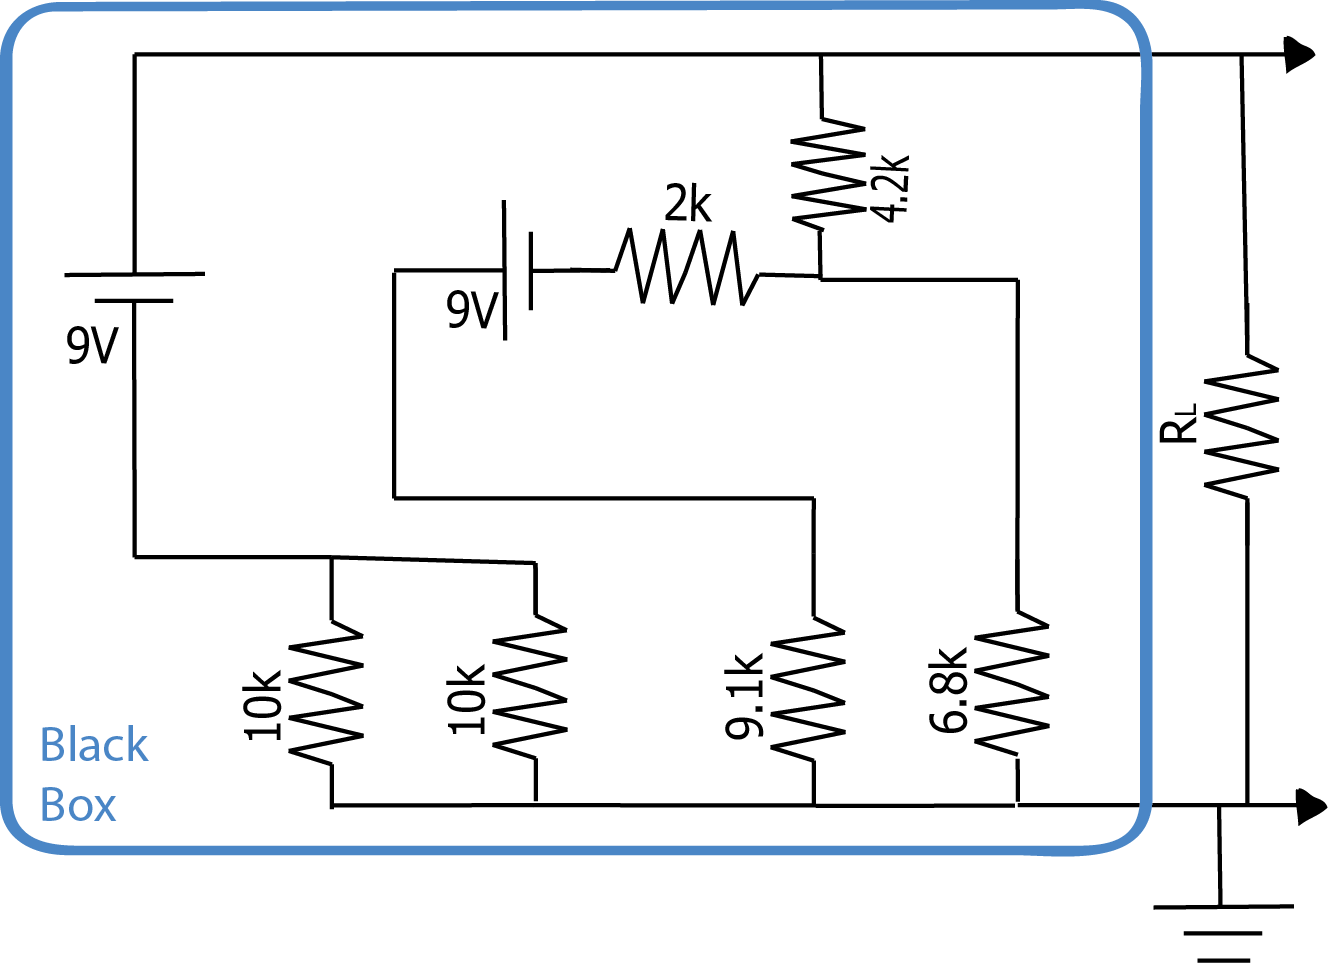
\includegraphics[width=200pt]{figure/thev_setup}
\caption{Using the resistor color chart, we decoded the resistor values  in the black box and computed the $V_{eq}$ and $R_{eq}$.}
\label{thev_setup}
\end{figure}
Since the battery is in parallel in the Thevenin circuit, the equivalent voltage is 9V. By decomposing the complicated Thevenin circuit into series and parallel parts, we can compute the equivalent resistance as 3.1367 k$\Omega$. Using Thevenin's theorem, since the components of the black box are all linear, we can simply treat everything in the Thevenin circuit (denoted by the blue box in Fig\ref{thev_setup}) as a single voltage source of $V_{eq}$ and resistor with $R_{eq}$. We used the measured the open-circuit voltage 4.1033V and the short circuit 1.2473mA to compute the Thevenin resistance:
\begin{equation}
R_{thev} = {V_{open}}{I_{short}}= \frac{4.1033V}{1.2473mA}=3.2897k\Omega
\end{equation}
which is within 5\% difference from the $R_{thev}$ computed from the nominal resistance values of the black box.
\begin{figure}[h!]
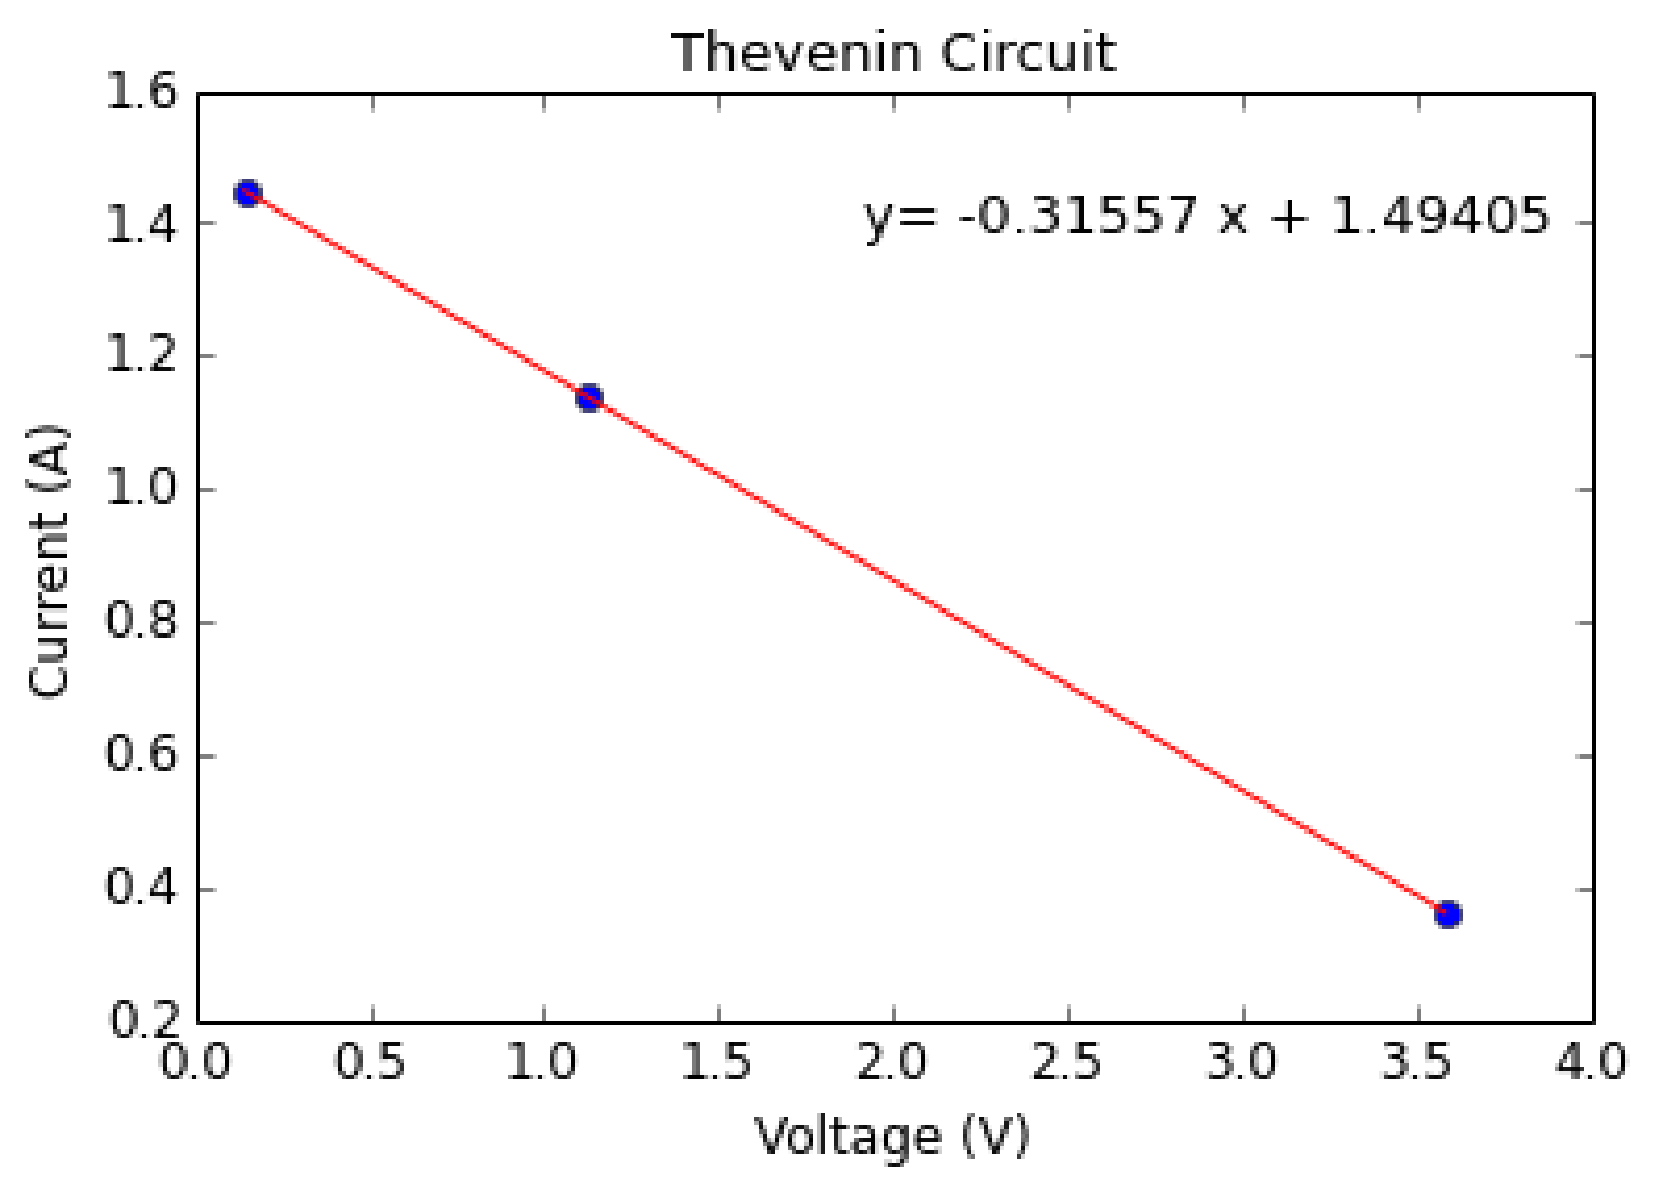
\includegraphics[width=200pt]{figure/thevenin}
%\caption{A straight-line fit through the data points for different values of load resistors shows that the output impedance is 0.32 $\Omega$.}
%\caption{The measurement of ------ slope is ---- , different values of load resistors. The measurement setup is illustrated in Fig. (REF!!).}
\caption{These voltages measurement accurately predict the trend that   as the load resistance increases, the current through the resistor decreases.}
\label{thevenin_plot}
\end{figure}
By shorting the battery with a jumper wire, we effectively bring the battery's terminals to equipotential, causing the output voltage to be 0V. The DMM measurement of resistance across the two terminals is 6.7k$\Omega$ which is 3.35k$\Omega\pm 0.442\Omega$.\footnote{Determined  by Eq.\ref{accuracy1_7} for the measurement and range of 1k$\Omega$. The computed $R_{thev}$ lies in this range.}
%%%%%%%%%%%%%%%%%%%%%%%%%%%%%%%%%%%%%%%%%%
\paragraph{\textbf{2.3}}
Here, we treat the oscilloscope as a black box of unknown impedance.  We substituted different resistors in the circuit shown in  Fig.\ref{Z_input}, and measured the input voltage. Using Eq.\ref{I_input}, we compute the input current as plotted in Fig. \ref{Z_input_plots}
\begin{equation}
I_{in} =\frac{V_{ext}-V_{in}}{R}
\label{I_input}
\end{equation}
From Eq.\ref{Z_in}, we see that the value of the slope is equivalent to the input impedance. A linear regression on the data results in a slope of 0.1978 M$\Omega\pm 8.24\times10^{-5}\Omega$. 
\begin{equation}
Z_{in}=\frac{V_{in}}{V_{ext}-V_{in}}R =\frac{V_{in}}{I_{in}}
\label{Z_in}
\end{equation}This result of a large input impedance makes sense since a larger impedance prevents the current to flow through easily, so that the oscilloscope does not perturb the circuit when conducting measurements.
%, which is the same order of magnitude as the input impedance of typical oscilloscope ( $\approx$ 1 M$\Omega$). \cite{tekronix}

%\subsection{2.1.14}
%$$Z_{out}=-\frac{\partial V}{\partial I}$$
%Given $v = 2/3c$, $\Delta$ d  = 10ft = 30.48m :
%\begin{equation}
%\Delta t = \frac{\Delta d}{v} = \frac{30.48m}{\frac{2}{3}\times 299792458 m/s} = 1.525 ns
%\end{equation}
%By comparing the difference between the signals in Fig. ----- peak-to-peak
\begin{figure}[h!]
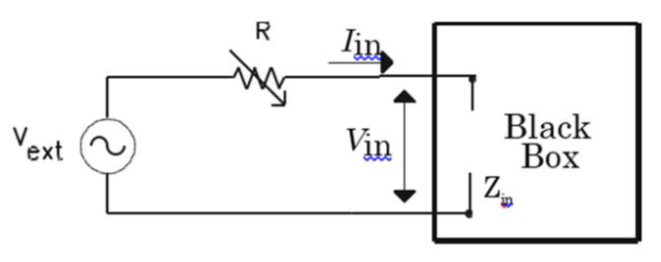
\includegraphics[width=200pt]{figure/d_Z_input}
\label{Z_input}
\caption{The circuit setup to find the $Z_{input}$ of the oscilloscope.}
\end{figure}
\begin{figure}[h!]
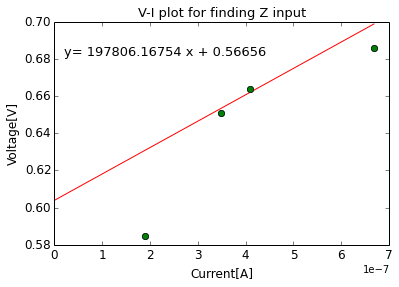
\includegraphics[width=200pt]{figure/Z_input_plot}
\caption{The uncertainty is computed according to Eq.\ref{accuracy1_7}, with range of 0.001V and 0.1mV for the last measurement. Since the error is on the order of magnitude of $10^{-5}$, the error bar plotted on this graph can not be seen unless zoomed in. }
\label{Z_input_plots}
\end{figure}
%%%%%%%%%%%%%%%%%%%%%%%%%%%%%%%%%%%%%%%%%%
\paragraph{\textbf{2.4}}

%%%%%%%%%%%%%%%%%%%%%%%%%%%%%%%%%%%%%%%%%%
\paragraph{\textbf{2.5}}

 \section{Conclusion}

fammilarize with settings, hands-on experience with equipment, including the DMM, breadboard, oscilloscope, black boxes and . Construct ------ , filters and ---- . 
\section*{Acknowledgments}
\begin{footnotesize}
The author would  like to acknowledge support from the GSI in this lab. I thank my partner, Leah Tom, for helpful discussion and collaboration that helped this work. We also appreciate Sissi Wong for helping us with the oscilloscope settings for question 1.2.7.
\end{footnotesize}
  \section*{References}
 \begin{footnotesize}
 \begin{itemize}
 \item Horowitz, Paul, and Winfield Hill. \textit{The Art of Electronics}. Cambridge: Cambridge UP, 1989. Print.
 \item ``Lab 1 - Introductory Experiments and Linear Circuits I." \textit{Donald A. Glaser Advanced Lab.} Regents of the University of California, n.d. Web. 01 Feb. 2015.
  \item ``Writing Lab Reports." \textit{Donald A. Glaser Advanced Lab.} Regents of the University of California, n.d. Web. 01 Feb. 2015.
% \item Press, William H., and William T. Vetterling. \textit{Numerical Recipes in C: The Art of Scientific Computing}. Cambridge University Press, 1992.  
\end{itemize}
% \bibliography{references}
%\bibliographystyle{elsarticle-harv}
  \end{footnotesize}

\end{document}
